\documentclass[11pt,preprint, authoryear]{elsarticle}

\usepackage{lmodern}
%%%% My spacing
\usepackage{setspace}
\setstretch{1.2}
\DeclareMathSizes{12}{14}{10}{10}

% Wrap around which gives all figures included the [H] command, or places it "here". This can be tedious to code in Rmarkdown.
\usepackage{float}
\let\origfigure\figure
\let\endorigfigure\endfigure
\renewenvironment{figure}[1][2] {
    \expandafter\origfigure\expandafter[H]
} {
    \endorigfigure
}

\let\origtable\table
\let\endorigtable\endtable
\renewenvironment{table}[1][2] {
    \expandafter\origtable\expandafter[H]
} {
    \endorigtable
}


\usepackage{ifxetex,ifluatex}
\usepackage{fixltx2e} % provides \textsubscript
\ifnum 0\ifxetex 1\fi\ifluatex 1\fi=0 % if pdftex
  \usepackage[T1]{fontenc}
  \usepackage[utf8]{inputenc}
\else % if luatex or xelatex
  \ifxetex
    \usepackage{mathspec}
    \usepackage{xltxtra,xunicode}
  \else
    \usepackage{fontspec}
  \fi
  \defaultfontfeatures{Mapping=tex-text,Scale=MatchLowercase}
  \newcommand{\euro}{€}
\fi

\usepackage{amssymb, amsmath, amsthm, amsfonts}

\usepackage[round]{natbib}
\bibliographystyle{natbib}
\def\bibsection{\section*{References}} %%% Make "References" appear before bibliography
\usepackage{longtable}
\usepackage[margin=2.3cm,bottom=2cm,top=2.5cm, includefoot]{geometry}
\usepackage{fancyhdr}
\usepackage[bottom, hang, flushmargin]{footmisc}
\usepackage{graphicx}
\numberwithin{equation}{section}
\numberwithin{figure}{section}
\numberwithin{table}{section}
\setlength{\parindent}{0cm}
\setlength{\parskip}{1.3ex plus 0.5ex minus 0.3ex}
\usepackage{textcomp}
\renewcommand{\headrulewidth}{0.2pt}
\renewcommand{\footrulewidth}{0.3pt}

\usepackage{array}
\newcolumntype{x}[1]{>{\centering\arraybackslash\hspace{0pt}}p{#1}}

%%%%  Remove the "preprint submitted to" part. Don't worry about this either, it just looks better without it:
\makeatletter
\def\ps@pprintTitle{%
  \let\@oddhead\@empty
  \let\@evenhead\@empty
  \let\@oddfoot\@empty
  \let\@evenfoot\@oddfoot
}
\makeatother

 \def\tightlist{} % This allows for subbullets!

\usepackage{hyperref}
\hypersetup{breaklinks=true,
            bookmarks=true,
            colorlinks=true,
            citecolor=blue,
            urlcolor=blue,
            linkcolor=blue,
            pdfborder={0 0 0}}


% The following packages allow huxtable to work:
\usepackage{siunitx}
\usepackage{multirow}
\usepackage{hhline}
\usepackage{calc}
\usepackage{tabularx}
\usepackage{booktabs}
\usepackage{caption}
\usepackage{colortbl}

\urlstyle{same}  % don't use monospace font for urls
\setlength{\parindent}{0pt}
\setlength{\parskip}{6pt plus 2pt minus 1pt}
\setlength{\emergencystretch}{3em}  % prevent overfull lines
\setcounter{secnumdepth}{5}

%%% Use protect on footnotes to avoid problems with footnotes in titles
\let\rmarkdownfootnote\footnote%
\def\footnote{\protect\rmarkdownfootnote}
\IfFileExists{upquote.sty}{\usepackage{upquote}}{}

%%% Include extra packages specified by user
% Insert custom packages here as follows
% \usepackage{tikz}

%%% Hard setting column skips for reports - this ensures greater consistency and control over the length settings in the document.
%% page layout
%% paragraphs
\setlength{\baselineskip}{12pt plus 0pt minus 0pt}
\setlength{\parskip}{12pt plus 0pt minus 0pt}
\setlength{\parindent}{0pt plus 0pt minus 0pt}
%% floats
\setlength{\floatsep}{12pt plus 0 pt minus 0pt}
\setlength{\textfloatsep}{20pt plus 0pt minus 0pt}
\setlength{\intextsep}{14pt plus 0pt minus 0pt}
\setlength{\dbltextfloatsep}{20pt plus 0pt minus 0pt}
\setlength{\dblfloatsep}{14pt plus 0pt minus 0pt}
%% maths
\setlength{\abovedisplayskip}{12pt plus 0pt minus 0pt}
\setlength{\belowdisplayskip}{12pt plus 0pt minus 0pt}
%% lists
\setlength{\topsep}{10pt plus 0pt minus 0pt}
\setlength{\partopsep}{3pt plus 0pt minus 0pt}
\setlength{\itemsep}{5pt plus 0pt minus 0pt}
\setlength{\labelsep}{8mm plus 0mm minus 0mm}
\setlength{\parsep}{\the\parskip}
\setlength{\listparindent}{\the\parindent}
%% verbatim
\setlength{\fboxsep}{5pt plus 0pt minus 0pt}



\begin{document}

\begin{frontmatter}  %

\title{Theory of Statistics Likelihood Assigment}

\author[Add1]{Sean Soutar STRSEA001}
\ead{sean.soutar@gmail.com}

\author[Add2]{Fabio Fehr FHRFAB001}
\ead{FHRFAB001@myuct.ac.za}




\address[Add1]{UCT Statistics Honours, Cape Town, South Africa}
\address[Add2]{UCT Statistics Honours, Cape Town, South Africa}


\begin{abstract}
\small{
This project will explore the Accidents dataset and try fit a Poisson,
Negative Binomial, Mixture of 2 Poissons and zero inflated Poisson
models to the data. The model with the strongest support will be chosen
and discussed. Profile likelihoods and confidence intervals for the
parameters will be found and displayed of the chosen model.
}
\end{abstract}

\vspace{1cm}

\begin{keyword}
\footnotesize{
Likelihood \sep Overdispersion \sep Soek \\ \vspace{0.3cm}
\textit{JEL classification} 
}
\end{keyword}
\vspace{0.5cm}
\end{frontmatter}



%________________________
% Header and Footers
%%%%%%%%%%%%%%%%%%%%%%%%%%%%%%%%%
\pagestyle{fancy}
\chead{}
\rhead{}
\lfoot{}
\rfoot{\footnotesize Page \thepage\\}
\lhead{}
%\rfoot{\footnotesize Page \thepage\ } % "e.g. Page 2"
\cfoot{}

%\setlength\headheight{30pt}
%%%%%%%%%%%%%%%%%%%%%%%%%%%%%%%%%
%________________________

\headsep 35pt % So that header does not go over title




\section{Introduction}\label{introduction}

This assignment is an explorative report on a dataset containing
accident counts. The aim of the report is to find and fit a model which
accurately describes the accident dataset. This report will first
explore the data then fit different adequate distributions and choose
the most appropriate one. Once a model has been selected the profile
likelihood and confidence intervals will be programmed and calculated
from from first principles. The results will then be analysed critically
and conclusions will be made and consider further considerations in the
study.

\subsection{Exploratory data analysis}\label{exploratory-data-analysis}

To better understand our data this report shall explore the following
properties; Firstly we examine the type of data within the accidents
dataset and discuss whether our data is discrete ordinal or continuous.
After the symmetry of the data and bounds will be discussed. This leads
the exploration to outliers and extreme values.

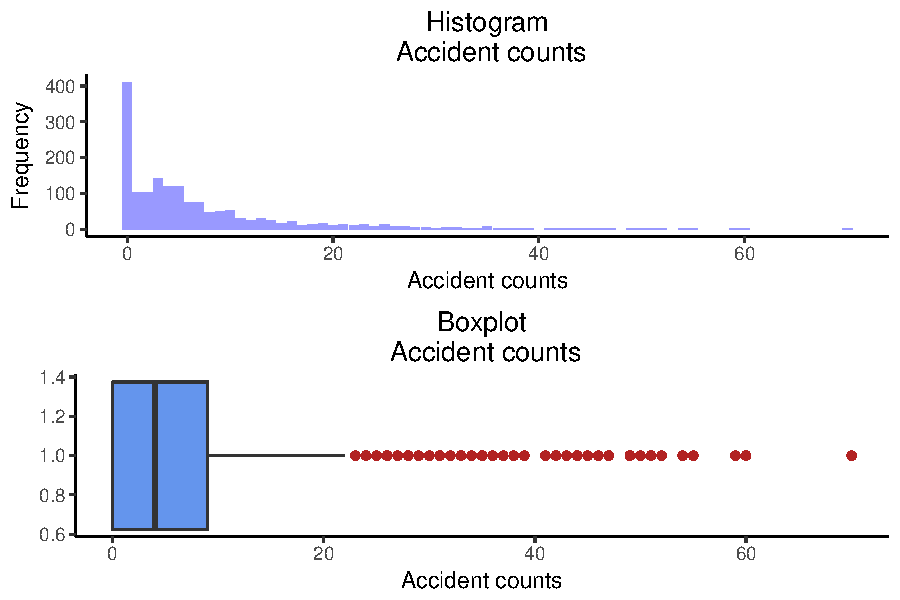
\includegraphics{likelihood_files/figure-latex/unnamed-chunk-1-1.pdf}

\subsubsection{Data type}\label{data-type}

The in our accident dataset we noticed that there are many observations
that have zero accidents. This suggests that we should focus on
distribution that are zero weighted. The accident counts are denoted as
a frequency which intuitively is a discrete variable and can take on
values greater than or equal to zero. Thus accident counts will be
regarded is a discrete positive definite random variable on the interval
\(R \in \{0;+ \infty\}\)

\subsubsection{Symmerty}\label{symmerty}

This property is visually seen in the histogram and boxplot displaying
the accident data. All count are greater than zero with the majority of
count being below 20. The largest accident count being 70. This shows
that the data is non symetrical and positively skewed.

\subsubsection{Outliers}\label{outliers}

From the boxplot it clear that many outliers exist. An observation is
termed an extreme value or outlier if it falls more than 1.5 times the
inner-quartile range above the upper quartile. The proportion of
outliers within our data set amount to 15.26\% this give us reason to
believe that population is also heavily skewed to the right. As
aforementioned there are observations more extreme than what is
displayed, which further reinforces our observation.

\section{Methods}\label{methods}

\subsection{Model Formulation}\label{model-formulation}

Since our data is discrete, asymmetric, positive definite, contains many
positive outliers and zeros this would suggest distributions such as
Poisson, Negative Binomial and mixture distributions such as 2 poisson
and a zero inflated Poisson.

\subsubsection{Poisson}\label{poisson}

\begin{align*} 
f(x) & = e^{-\lambda} \frac{\lambda^x}{x!},\ \ x\in \{0,1,\ldots,\infty\},\lambda>0 \\
\\
L(\lambda|x) & = \prod_{i=1}^n f(x_i) \\
\\
L(\lambda|x) & =e^{-n\lambda}\dfrac{\lambda^{\sum_{i=1}^n x_i}}{\prod_{i=1}^n x_i!}\\
\\
l(\lambda|x) & =-n\lambda +  \left(\sum_{i=1}^n x_i\right)\ln \lambda + \ln(\prod_{i=1}^n x_i!).
\end{align*}

-define all parameters -fit to the data

\subsubsection{Negative Binomial}\label{negative-binomial}

\begin{align*}
f(x) & = \left( \begin{array}{c}
x+j-1  \\
x  \end{array} \right)(1-\pi)^x\pi^j,\ \ x,\in \{0,1,\ldots,\infty\}, 0 \leq \pi \leq 1\\
\\
L(\lambda|x) & = \prod_{i=1}^n f(x_i) \\
\\
L(\lambda|x) & = \prod_{i=1}^n \left( \begin{array}{c}
x_i+j-1  \\
x_i  \end{array} \right)(1-\pi)^{\sum_{i=1}^n x_i}\pi^{nj}\\
\\
l(\lambda|x) & = \sum_{i=1}^n \ln \left( \begin{array}{c}
x_i+j-1  \\
x_i  \end{array} \right)+{\sum_{i=1}^n x_i} \ln (1-\pi) + {nj} \ln(\pi)
\end{align*}

-define all parameters -fit to the data

\subsubsection{Mixture of 2 poissons}\label{mixture-of-2-poissons}

-Likelihood -define all parameters -loglikelihood

-fit to the data

-Here I am assuming the mixture will be poisson with rate = sample mean
and the other poisson will have a rate of 0.1 to take into account the
zero inflation ?

\subsubsection{Zero inflated Poisson}\label{zero-inflated-poisson}

-Likelihood -loglikelihood -define all parameters -fit to the data -We
can use optimisers but we must program the likelihoods ourselves

\subsection{Model Selection}\label{model-selection}

-compare models and choose the best one -Illustrate how good the model
is

-We need to reparameterize parameters so that they are unbounded

\subsection{Profile Likelihood \& Confidence
Intervals}\label{profile-likelihood-confidence-intervals}

-Plot likelihood surface (two parameters at a time if necessary, fixing
the other parameters at their MLEs).

-Must be program the profile likelihoods, CI's ourselves

\section{Results}\label{results}

\section{Conclusion}\label{conclusion}

-What are the next steps and how can we improve the models

\section{References}\label{references}

% Force include bibliography in my chosen format:
\newpage
\nocite{*}
\bibliography{}





\end{document}
